\documentclass{article}
\usepackage{stackengine}
\usepackage{graphicx}
\usepackage{amsmath}
\usepackage{cite}
\title{Lecture 1: Introduction}
\author{Shashank Vatedka}

\usepackage{basicreq}
\usepackage{./teaching_doc_macros}

\begin{document}
	
	%FILL IN THE RIGHT INFO.
	%\lecture{**LECTURE-NUMBER**}{**UNIT**}{**LECTURER**}{**SCRIBE**}
	\lecture{11}{Tools for proving converse results}{Shashank Vatedka}{Ritesh Kumar}
	%\footnotetext{These notes are partially based on those of Nigel Mansell.}
	
	% **** YOUR NOTES GO HERE:
	
	% Some general latex examples and examples making use of the
	% macros follow.  
	%**** IN GENERAL, BE BRIEF. LONG SCRIBE NOTES, NO MATTER HOW WELL WRITTEN,
	%**** ARE NEVER READ BY ANYBODY.

\section{Fano's inequality}
Consider M and $\hat{M}$ are jointly distributed and probability of error $P_e = Pr[M \neq \hat{M}]$. And M \& $\hat{M}$
 $\in \mathbb{M}$. Then 
 
\begin{equation}
	H(M/\hat{M}) \leq H_2 (P_e ) + P_e \text{log}|\mathbb{M}|
	\end{equation}
 
 Proof : \\
 Consider a indicator function  E as :
 \begin{equation}
 	E = \left\{\begin{matrix}
 	1 	& \text{if}  \hspace{5pt}\hat{M} \neq  M \\ 
 	0	&  \text{if} \hspace{5pt} \hat{M} = M
 	\end{matrix}\right.
 \end{equation}
 So,we have $P_E(1)= P_e , P_E(0) = 1 -P_e$, and we can write $H(E) = H_{2}(P_e)$. Now
\begin{gather}
H \left (M,E|\hat{M} \right) = H \left (M|\hat{M} \right ) + H \left(E|M, \hat{M} \right) \text{ (chain rule of entropy)}\\
\hspace*{-9mm}H \left(M|\hat{M} \right)  = H \left( E|\hat{M}\right) +  H \left( E|M, \hat{M} \right) - H\left( E|M\hat{M} \right)
\end{gather} 
Since E is independent from M and $\hat{M}$, we can write, 
\begin{gather}
\hspace*{-6.5cm} H \left(M| \hat{M}\right)  = H \left( E|\hat{M} \right) +  H \left( \frac{M}{E}, \hat{M} \right)\\
\hspace*{-5.5cm} \leq  H\left( E\right) +   H \left( M|E, \hat{M} \right) \\
 = H_{2}\left( P_e\right) +   H \left( M| \hat{M}, E=0 \right) P_E(0) +  H \left( M| \hat{M}, E=1 \right) P_E(1)
\end{gather}
Here,  $ H \left( M| \hat{M}, E=0 \right) = 0$ because for E = 0 , M = $\hat{M}$, and hence entropy = 0.
 \begin{gather}
\hspace*{.5cm} = H_{2}\left( P_e\right) +  H \left( M| \hat{M}, E=1 \right) P_E(1)\\
 = H_{2}\left( P_e\right) +  H \left( M| \hat{M}, E=1 \right) P_e\\
\hspace*{-1.3cm} \leq  H_{2}\left( P_e\right) +  H \left(M\right) P_e\\
\hspace*{.2cm} \leq  H_{2}\left( P_e\right) +  P_e \text{log}_{2}|\mathbb{M}|\hspace*{2mm} \text{Proved.}
 \end{gather}
 \section{Proof of converse channel coding theorem}

\textbf{Theorem :} Consider any sequence with (ENC$_{n}$, DEC$_{n}$) for DMC with transition probability P$_{Y|X}$ such that ,\\
\begin{eqnarray*}
 \stackunder{$\liminf$}{n$\rightarrow \infty$} \frac{K_n}{n} \geq C + \epsilon
 \end{eqnarray*}
 then, 
 \begin{eqnarray*}
 	 P_{e} = \stackunder{$\limsup$ }{$n$ $\rightarrow$ $\infty$} =  Pr \left [ \hat{M}_{i} \neq M_{i} \right ] \geq \frac{\epsilon}{R}
 \end{eqnarray*} 
 \begin{figure}[h!]
  \centering
 \includegraphics[height=.10\textheight]{pic6.pdf}
 \caption{ Single user over DMC }
 \label{fig11.1}
 \end{figure}
 
\textbf{Proof:} \\ We need some well-known inequalities to prove this. 1) Fano's inequality and 2) bound on mutual information. Fano's inequality we have discussed just above and now let us discuss bound on mutual information.\\
\textbf{Lemma :} \hspace{1mm}For any P$_{X^n}$, if Y$^{n}$ is obtained by passing  X$^{n}$ through Discrete memoryless channel having transition probability P$_{Y|X}$  then,
\begin{equation}
	I \left( X^n ; Y^n\right) \leq \sum_{i=1}^{n} I \left( {X_i ; Y_i} \right) \leq nC \label{11.12}
\end{equation}
 \textbf{Proof of lemma :}\\\\
Consider the expression of mutual information,
 \begin{gather}
 	I\left( X^n; Y^n\right) = H \left( Y^n\right) - H \left( Y^n|X^n\right) \label{11.13}\\
 = \sum_{i =1}^{n} \left[ H \left(Y_i|Y_1, Y_2 \dots Y_{i-1}\right) - H \left( Y_i|Y_1, Y_2 \dots Y_{i-1}, X^n \right)\right] \label{11.14}
 \end{gather}
 	\hspace{10cm} $\left( \text{Chain rule of entropy}\right)$	
 	\begin{gather}
 	\leq \sum_{i=1}^{n} \left[ H\left( Y_i\right) - H\left( Y_i|Y_1, Y_2 \dots Y_{i-1}, X^n \right) \right] \label{11.15}
 	\end{gather}
 	\hspace{10cm} $\left( \text{Since conditioning decreases  entropy}\right)$\\ 
 Now,
 \begin{equation}
 H \left( Y_i|Y_1, Y_2 \dots Y_{i-1}, X^n \right)   =  \sum_{x^n, y_1, \dots , y_n} P_{Y|X}\left( y_i|y_1, \dots y_{i-1}, x^n \right) \times \text{log}\left( \frac{1}{P_{Y|X}\left( y_i|y_1, \dots y_{i-1}, x^n \right)}  \right) \label{11.16}
 \end{equation}
 	Since for discrete memoryless channel present output depends only on the present input, hence we can write.
 	\begin{equation}	
 P_{Y|X}\left( y_i|y_1, \dots y_{i-1}, x^n \right) =   P_{Y|X}\left( y_i |x_i, y_1,x_i \dots y_{i-1},x_{i-1} \right) =  P_{Y|X}\left( y_i | x_i \right) \label{11.17}
 \end{equation}
Using eq \eqref{11.17} in eq \eqref{11.16}, we can write,
 	\begin{equation}
  H \left( Y_i|Y_1, Y_2 \dots Y_{i-1}, X^n \right) =  \sum_{x^n, y_1, \dots , y_n} P_{Y|X}\left( y_i|x_i \right) \times \text{log}_{2}\left(  \frac{1}{ P_{Y|X}\left( y_i| x_i \right)}\right) = 	H \left( Y_i|X_i \right) \label{11.18}	
 \end{equation}
  By combining all i.e using eq\eqref{11.18} in eq\ref{11.15} we can write,
  \begin{equation}
  = \sum_{i=1}^{n} \left[ H\left( Y_i\right) - H \left( Y_i| X_i \right) \right]
  \end{equation}
 And we have,
 \begin{equation}
 	 \sum_{i=1}^{n} \left[ H\left( Y_i\right) - H\left( Y_i |X_i \right) \right] = \sum_{i=1}^{n} I \left( {X_i ; Y_i} \right) \label{11.20}
 \end{equation}
From  eq\eqref{11.13}, eq\eqref{11.15} and eq\eqref{11.20} we have,
\begin{equation}
	I \left( X^n ; Y^n\right) \leq \sum_{i=1}^{n} I \left( {X_i ; Y_i} \right) \leq nC \label{11.21}
\end{equation}
This conclude the proof of eq \eqref{11.12}. \\

\textbf{Proof of converse:}


We have message, which is i.i.d and uniform so we can write,
\begin{gather}
	K_n = H \left( M^{K_n}\right)\\
	= H\left( M^{K_n}|\hat{M}^{K_n}\right) + I\left( M^{K_n} ; \hat{M}^{K_n}\right)\\
   \leq H_{2}(P_{e}) + P_{e}\text{log}_{2}(2^{M^{K_{n}}}) + I(M^{K_{n}}:{M'}^{K_{n}})
\end{gather}
\hspace{10cm} $\left(\text{ using Fano's inequality} \right)$
\begin{gather}
	\leq H_{2}\left( P_e\right) + P_{e}K_{n} + I\left( M^{K_n} ; \hat{M}^{K_n}\right)
\end{gather}

\begin{equation}
	\leq H_{2}\left( P_e\right) + P_{e}K_{n} + I\left( X^n ; Y^n\right)
\end{equation}
\hspace{10cm} $\left(\text{ using data processing inequality} \right)$
\begin{equation}
	\leq H_{2}\left( P_e\right) + P_{e}K_{n} + nC  \hspace{2mm}\text{ (From eq \ref{11.21} )}
\end{equation}
\begin{eqnarray*}
	  	K_{n}  \leq H_{2}(P_{e}) + P_{e}K_{n} + nC  \Rightarrow \frac{H_{2}(P_{e})}{n} \geq \frac{K_{n}(1 - P_{e})}{n} - C \\
	 	\stackunder{$\lim$ }{$n$ $\rightarrow$ $\infty$} \left(  \frac{K_{n}(1 - P_{e})}{n} - C \right) \leq  \stackunder{$\lim$ }{$n$ $\rightarrow$ $\infty$} \frac{H_{2}(P_{e})}{n}  
	 \end{eqnarray*} 

Where, P$_{e} = \stackunder{$\limsup$ }{$n$ $\rightarrow$ $\infty$} Pr \left[ \hat{M}_{i}^{K_n} \neq M_{i}^{K_n}\right]$ \newpage
Let $\frac{K_{n}}{n} = R $, \\
 
\begin{align}
\stackunder{$\lim$}{$n$ $\rightarrow$ $\infty$} P_{e} \geq \frac{R - C}{R} 
\end{align}
 
 \begin{align}
 	\stackunder{$\limsup$}{$n$ $\rightarrow$ $\infty$} P_{e} \geq \frac{R - C}{R} \label{2.15}
 \end{align} 
  
  If we operate at the rate more than capacity of the channel say R = C + $\epsilon$
  \begin{align}
  	\stackunder{$\limsup$}{$n$ $\rightarrow$ $\infty$} \hspace{5pt} P_{e} \geq \frac{\epsilon}{R} 
  \end{align}
\begin{figure}[h!]
	\centering
	\includegraphics[height=.20\textheight]{pic7.pdf}
	\caption{Probability of error with capacity constraint }
	\label{fig11.2}
\end{figure}
That is probability or error  is always non-zero.But if we operate the channel  below the capacity and for large n, in \eqref{2.15} we can observe P$_{e}$  approaches to 0.  
  
  \section{Mrs Gerber's Lemma:}

Suppose we have X = $\left( X_i, \dots X_n\right)$ where X$_{i} \in \mathbb{M}^{{n}} \in \left \{ 0,1\right \}$
 be a binary random n-vector.
Let P$_{X}(x)= P\left( X = x \right)$, where $x \in \mathbb{M}^{n}$  define its probability distribution Let say X $\sim$ Ber(q). Let us consider that the random vector X is the input to a binary symmetric channel with crossover probability  p, where $0 < p < \frac{1}{2}$.
\begin{figure}[h!]
	\centering
	\includegraphics[height=.12\textheight]{pic8.pdf}
	\caption{BSC channel }
	\label{fig11.3}
\end{figure}
 Let  be  Y = $\left( Y_i, \dots Y_n\right)$ where Y$_{i} \in \mathbb{M}^{{n}} \in \left \{ 0,1\right \}$
the corresponding channel output n-vector. The probability
distribution of Y is defined using transition probability of channel and X $\left( \text{described in figure \ref{fig11.3}} \right)$.
We will use notation \textbf{p$\star$q = p(1-q) + q(1-p)}. Then ,
\begin{equation}
	H(Y) \geq H_{2}\left( p \star H_{2}^{-1} \left( H(X)\right)\right) \label{11.31}	
\end{equation}		
with equality if and only if the ${\left\{X_{i}\right \}_{1}}^{n}$ are independent. and H$\left\{ X^k
\right\} = kp$ 

\textbf{Lemma :} \hspace{1mm} Suppose we are generating X which depends on some distribution U, and it passes through BSC(p) (with transition probability p) with output distribution Y. Then,
\begin{equation}
	H\left(\frac{Y}{U}\right) \geq H_2\left( H_{2}^{-1}\left( H\left( \frac{X}{U}\right)\right) \star p\right)
\end{equation}
\begin{figure}[h!]
	\centering
	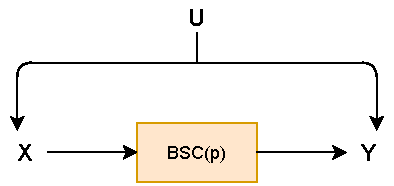
\includegraphics[height=.12\textheight]{pic9.pdf}
	\caption{Binary symmetric channel }
	\label{fig11.4}
\end{figure}

In vector form,
\begin{equation}
	\frac{H\left( Y^{n}|U \right)}{n} \geq H_2\left( H_{2}^{-1}\left( H\left(\frac{ X^{n}|U}{n}\right)\right) \star p\right)
\end{equation}

\begin{proof}
We have claim ,
\begin{equation}
	H\left(\frac{Y}{U}\right) \geq H_2\left( H_{2}^{-1}\left( H\left( \frac{X}{U}\right)\right) \star p\right)
\end{equation}
Considering R.H.S. of the inequality we have, 
\begin{equation}
 H_2\left( H_{2}^{-1}\left( H\left( \frac{X}{U}\right)\right) \star p\right) \label{11.35}
\end{equation}
Suppose we have $f(u) = H_{2} \left( H_{2}^{-1}(v)\star p\right)$.\\
Now, eq \eqref{11.35} can be written as, 
\begin{equation}	
f \left( \sum_{u} P_{U}(u). H \left( X | U = u\right)\right)
\end{equation}
 \textbf{Claim :} $f$ is convex function. 
 \begin{proof}
 	We have $f(u) = H_{2} \left( H_{2}^{-1}(v)\star p\right)$.
 Let consider, $ g(u) = H_{2}^{-1}(v),$\\ 
 Then, we can write,
 \begin{eqnarray*}
 f(u) = H_{2} \left(g(u)\star p\right),\\
 f(u) = H_{2} \left( g(u)(1-p) + \left(1-g(u)\right)p\right)	
 \end{eqnarray*}
put $\alpha = g(u)(1-p) + \left(1-g(u)\right)p $, so we have,
 \begin{eqnarray*}
	f(u) = H_{2} \left( \alpha \right)= - \left[ \alpha \log_{2}(\alpha) + (1-\alpha) \log_{2}(1-\alpha)\right]	\\
	f'(u) = - \left[ \frac{\alpha}{\alpha} + \log_{2}\alpha \frac{1-\alpha}{ 1-\alpha} (-1) + (-1) \log_{2}(1-\alpha)\right] \frac{1}{\ln(2)}. \frac{\partial \alpha }{\partial u}  \\
	f'(u) = - \frac{1}{\ln(2)}.g'(u)(1-2p) \left[ \log (\frac{\alpha}{1- \alpha})\right]\\
	f''(u) = \frac{1}{\ln(2)}.g''(u)(1-2p)^2 \left[  \frac{2- \alpha}{\alpha (1 -\alpha)}\right]
\end{eqnarray*}	
 Here $f''(u)$ is always positive for $0< \alpha <1$, hence $f$ is convex function.		
 	\end{proof}
 Now coming to main proof of lemma.
Since $f$ is convex function, we can write,
\begin{equation}
f \left( \sum_{u} P_{U}(u). H \left( X | U = u\right)\right) \leq   \sum_{u} P_{U}(u). f \left(H \left( X | U = u\right)\right) 
\end{equation}
Again using the expression of $f(u)$ we can have,
\begin{equation}
	f\left(H\left( X|U=u\right)\right) =  H_{2} \left( H_{2}^{-1}\left(H\left( X|U=u\right)\right)\star p\right)
\end{equation}
 For $U = u, X \sim $ Ber$(q_{u})$ and Y $\sim (q_{u} \star p)$.
 \begin{equation}
 H\left( X|U=u\right) = H_{2}\left(q-{u} \star p\right) = H_{2} \left( H_{2}^{-1}\left(H\left( X|U=u\right)\right)\star p\right) = 	f\left(H\left( X|U=u\right)\right)
 \end{equation} 
Combining all above expressions, R.H.S. becomes, 
\begin{equation}
	\text{R.H.S} \leq  \sum_{u} P_{U}(u). H \left( X | U = u\right)
\end{equation}
Hence,
\begin{equation}
	H\left(\frac{Y}{U}\right) \geq H_2\left( H_{2}^{-1}\left( H\left( \frac{X}{U}\right)\right) \star p\right)
\end{equation}
and this concludes the proof.
\end{proof}

\end{document}

